\documentclass[twoside]{article}
\usepackage[a4paper]{geometry}
\geometry{verbose,tmargin=2.5cm,bmargin=2cm,lmargin=2cm,rmargin=2cm}
\usepackage{fancyhdr}
\pagestyle{fancy}

% nastavení pisma a~češtiny
\usepackage{lmodern}
\usepackage[T1]{fontenc}
\usepackage[utf8]{inputenc}
\usepackage[czech]{babel}

% odkazy
\usepackage{url}

\usepackage{float}
% vícesloupcové tabulky
\usepackage{multirow}
\usepackage{listings}
\usepackage{xcolor}
\usepackage{amssymb}
\usepackage{gensymb}
\usepackage{bbold}
\usepackage{amsmath}
\usepackage{siunitx}
\usepackage{mathtools}
\usepackage{commath}

% vnořené popisky obrázků
\usepackage{subcaption}

% automatická konverze EPS 
\usepackage{graphicx} 
\usepackage{epstopdf}
\epstopdfsetup{update}

\graphicspath{{./images}}

% odkazy a~záložky
\usepackage[unicode=true, bookmarks=true,bookmarksnumbered=true,
bookmarksopen=false, breaklinks=false,pdfborder={0 0 0},
pdfpagemode=UseNone,backref=false,colorlinks=true] {hyperref}


% Poznámky při překladu
\usepackage{xkeyval}	% Inline todonotes
\usepackage[textsize = footnotesize]{todonotes}
\presetkeys{todonotes}{inline}{}

%https://tex.stackexchange.com/questions/2783/bold-calligraphic-typeface
\DeclareMathAlphabet\mathbfcal{OMS}{cmsy}{b}{n}

% enumerate zacina s pismenem
\renewcommand{\theenumi}{\alph{enumi}}

% smaz aktualni page layout
\fancyhf{}
% zahlavi
\usepackage{titling}
\fancyhf[HC]{\thetitle}
\fancyhf[HLE,HRO]{\theauthor}
\fancyhf[HRE,HLO]{\today}
 %zapati
\fancyhf[FLE,FRO]{\thepage}

% údaje o autorovi
\title{OTE Domácí úkol 4a - Integrační zesilovač}
\author{Vojtěch Michal}
\date{\today}

%customize code listing
\definecolor{codegreen}{rgb}{0,0.6,0}
\definecolor{codegray}{rgb}{0.5,0.5,0.5}
\definecolor{codepurple}{rgb}{0.58,0,0.82}
\definecolor{backcolour}{rgb}{0.95,0.95,0.92}

\lstdefinestyle{mystyle}{
    backgroundcolor=\color{backcolour},   
    commentstyle=\color{codegreen},
    keywordstyle=\color{magenta},
    numberstyle=\tiny\color{codegray},
    stringstyle=\color{codepurple},
    basicstyle=\ttfamily\footnotesize,
    breakatwhitespace=false,         
    breaklines=true,                 
    captionpos=b,                    
    keepspaces=true,                 
    numbers=left,                    
    numbersep=5pt,                  
    showspaces=false,                
    showstringspaces=false,
    showtabs=false,                  
    tabsize=2
}

\lstset{style=mystyle}

\begin{document}

\maketitle

V simulacích pro tuto úlohu bylo použito nastavení parametrů operačního zesilovače uvedené v tabulce \ref{tab:oz_param}.
Symbolem $u_2$ označuji napětí na výstupu integračního zesilovače proti zemi,
napětí $u_1$ je napětí na vstupu do integrátoru proti zemi
(konvence použitá v zadání). Struktura integračního zesilovače je na obrázku \ref{fig:int_amp}.

\begin{table}[h!]
    \centering
    \begin{tabular}{c|c|c|c|c}
        parametr & symbol & hodnota & jednotka & poznámka\\
        \hline
        Vstupní napěťový offset & $U_0$ & 1 & \si{\milli\volt} & \\
        Vstupní klidový proud & $I_\text{B}$ & 50 & \si{\nano\ampere} & $(I_\text{BP} + I_\text{BN})/2$ \\
        Vstupní zbytkový proud & $I_0$ & 20 & \si{\nano\ampere} & $I_\text{BP} - I_\text{BN}$ \\
        Zesílení v otevřené smyčce & $A_\text{D}$ & 200 & \si{\kilo\volt\per\volt} & \\
        Tranzitní kmitočet& $f_T$ & 1 & \si{\mega\hertz} &
    \end{tabular}
    \caption{Parametry operačního zesilovače použité pro simulaci}
    \label{tab:oz_param}
\end{table}

\begin{figure}[h!]
    \centering
    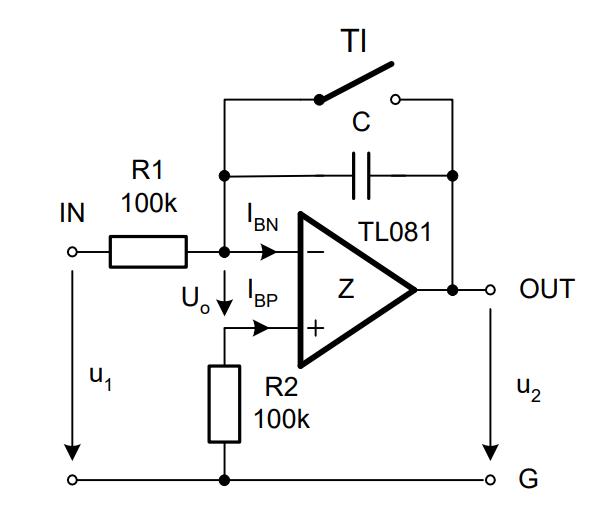
\includegraphics[width=0.5\linewidth]{int_amp.png}
    \caption{Struktura invertujícího integračního zesilovače, převzato ze zadání}
    \label{fig:int_amp}
\end{figure}


\section{Výpočet časové konstanty}

Pro časovou konstantu integrátoru platí
\begin{equation}
    \tau = R_1 C,
\end{equation}
fixováním $R_1 = 100 \si{\kilo\ohm}$ lze pro proměnné velikosti $C$ dosáhnout
různé časové konstanty dle tabulky \ref{tab:tau}. Pro kompletnost jsou v tabulce uvedeny i příslušné mezní frekvence
vypočtené dle vztahu
\begin{equation}
    f = \frac{\omega}{2 \pi} = \frac{1}{2 \pi \tau}= \frac{1}{2 \pi R_1 C}.
\end{equation}

\begin{table}[h!]
    \centering
    \begin{tabular}{c|c|c}
        $C_1$ & Časová konstanta $\tau$ &mezní frekvence $f_m$\\
        \hline
        1 \si{\nano\farad} & 100 \si{\micro\second} & 1,59 \si{\kilo\hertz}\\
        10 \si{\nano\farad} & 1\si{\milli\second} & 159 \si{\hertz}\\
        100 \si{\nano\farad} & 10 \si{\milli\second} & 15,9 \si{\hertz}\\
        1 \si{\micro\farad} & 100 \si{\milli\second} & 1,59 \si{\hertz}
    \end{tabular}
    \caption{Závislost časové konstanty integrace na kapacitě $C_1$}
    \label{tab:tau}
\end{table}

\section{Zbytková napětí}

Zkratováním vstupu na zem dle schématu \ref{fig:zbytkove_u} se projevuje vstupní zbytkové napětí OZ samotného a
integrované napětí diverguje do nekonečna (na napájení úrovně).

\begin{figure}[h!]
    \centering
    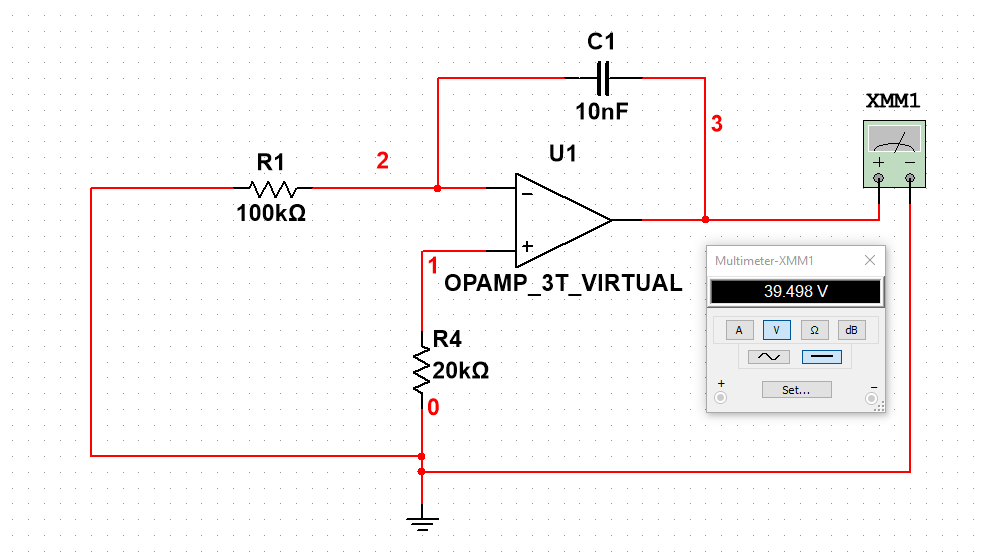
\includegraphics[width=0.65\linewidth]{zbytkove_u.png}
    \caption{Schéma pro měření výstupního zbytkového napětí}
    \label{fig:zbytkove_u}
\end{figure}

Zapojením zpětné vazby kolem integrátoru dle schématu \ref{fig:vstupni_zbytkove} lze nalézt i jeho vstupní zbytkové napětí,
při kterém se $u_2$ bude držet na zemním potenciálu. To je pro mé parametry OZ rovno $U_0 = 3\si{\milli\volt}$.

\begin{figure}[h!]
    \centering
    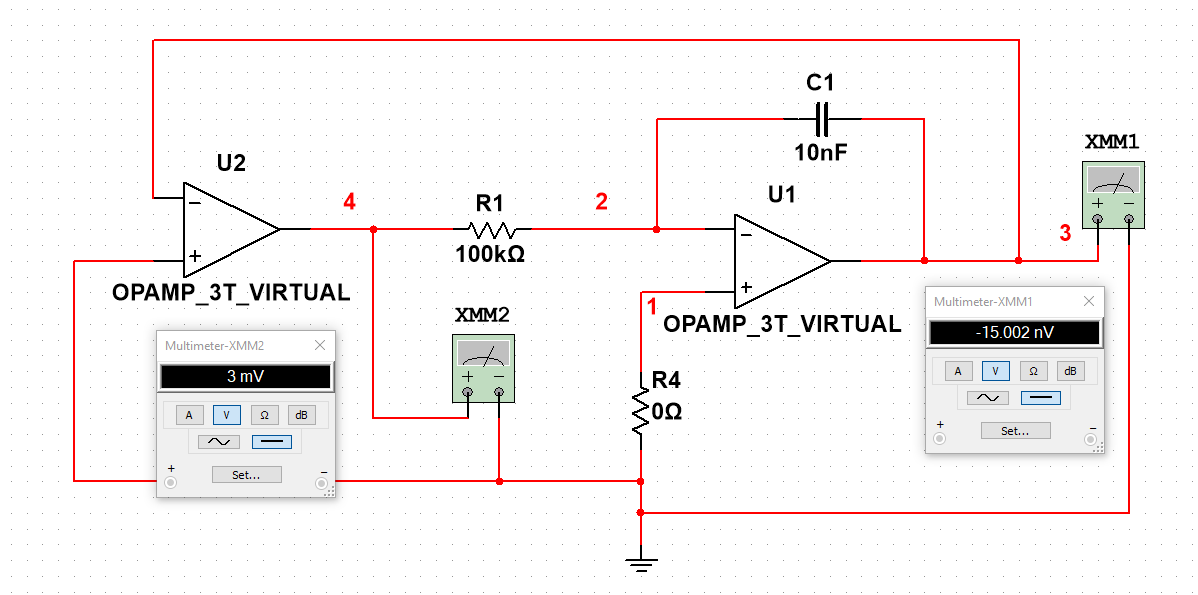
\includegraphics[width=0.65\linewidth]{vstupni_zbytkove.png}
    \caption{Schéma pro měření vstupního zbytkového napětí}
    \label{fig:vstupni_zbytkove}
\end{figure}

\newpage
\section{Frekvenční charakteristika}

S pomocí zapojení na schématu \ref{fig:schema_bode} a funkce \textit{AC sweep} byly
získány frekvenční charakteristiky integračního zesilovače pro $C_1 \in \left\{1, 100\right\} \si{\nano\farad}$,
které jsou vykresleny na obrázkách \ref{fig:bode_1} a \ref{fig:bode_100}.
Simulací určené mezní kmitočty odpovídají přesně teoreticky vypočteným hodnotám v tabulce \ref{tab:tau}.

\begin{figure}[h!]
    \centering
    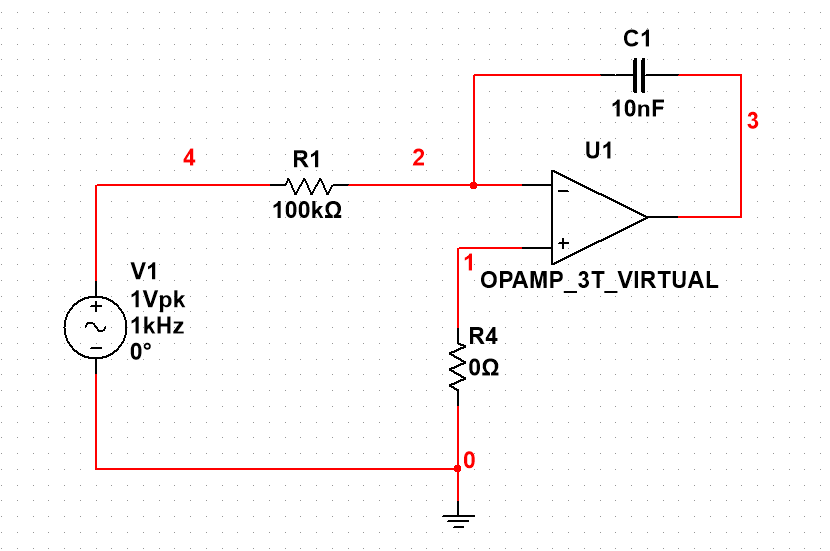
\includegraphics[width=0.8\linewidth]{bode_schema.png}
    \caption{Zapojení pro získání frekvenční charakteristiky integračního zesilovače}
    \label{fig:schema_bode}
\end{figure}

\newpage
\begin{figure}[h!]
    \centering
    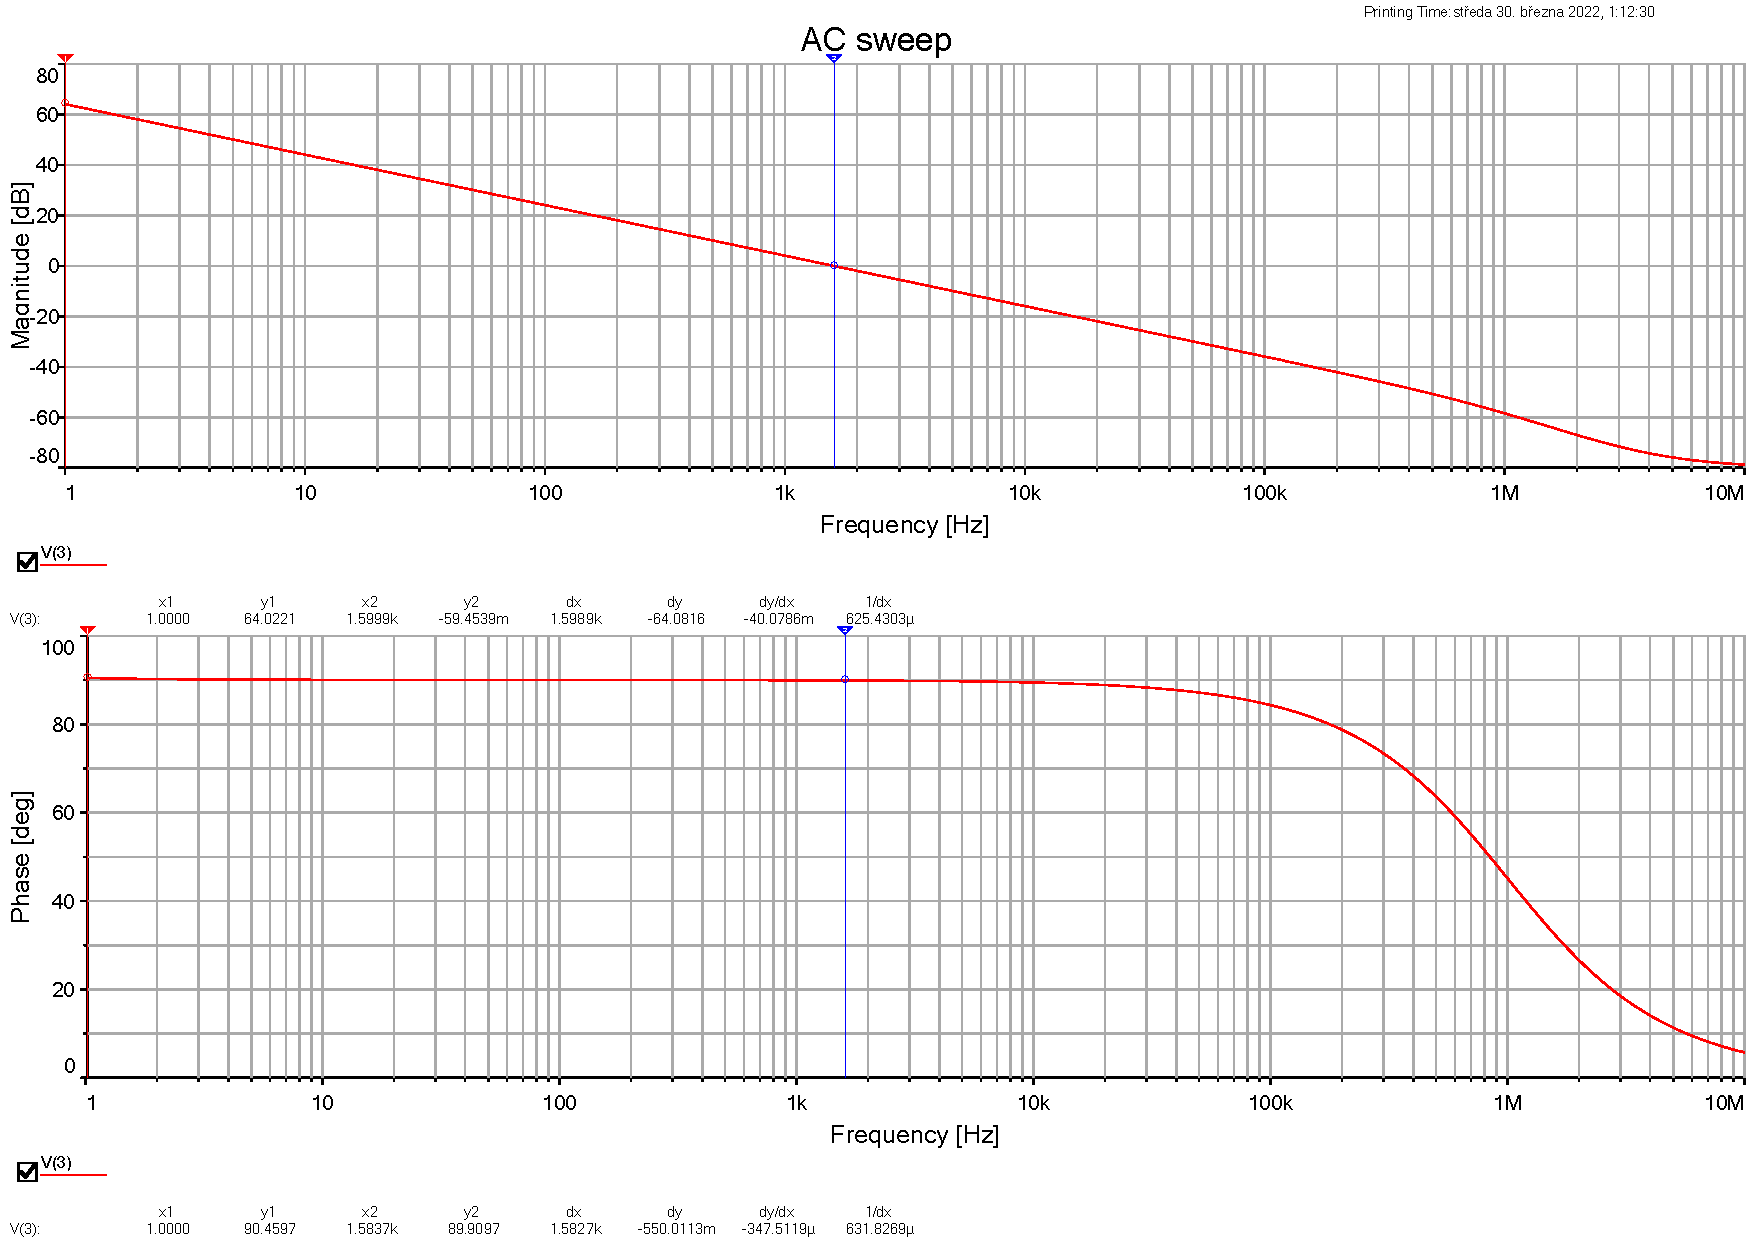
\includegraphics[width=0.92\linewidth]{bode_1.pdf}
    \caption{Frekvenční charakteristika pro $C_1 = 1 \si{\nano\farad}$}
    \label{fig:bode_1}
\end{figure}

\begin{figure}[h!]
    \centering
    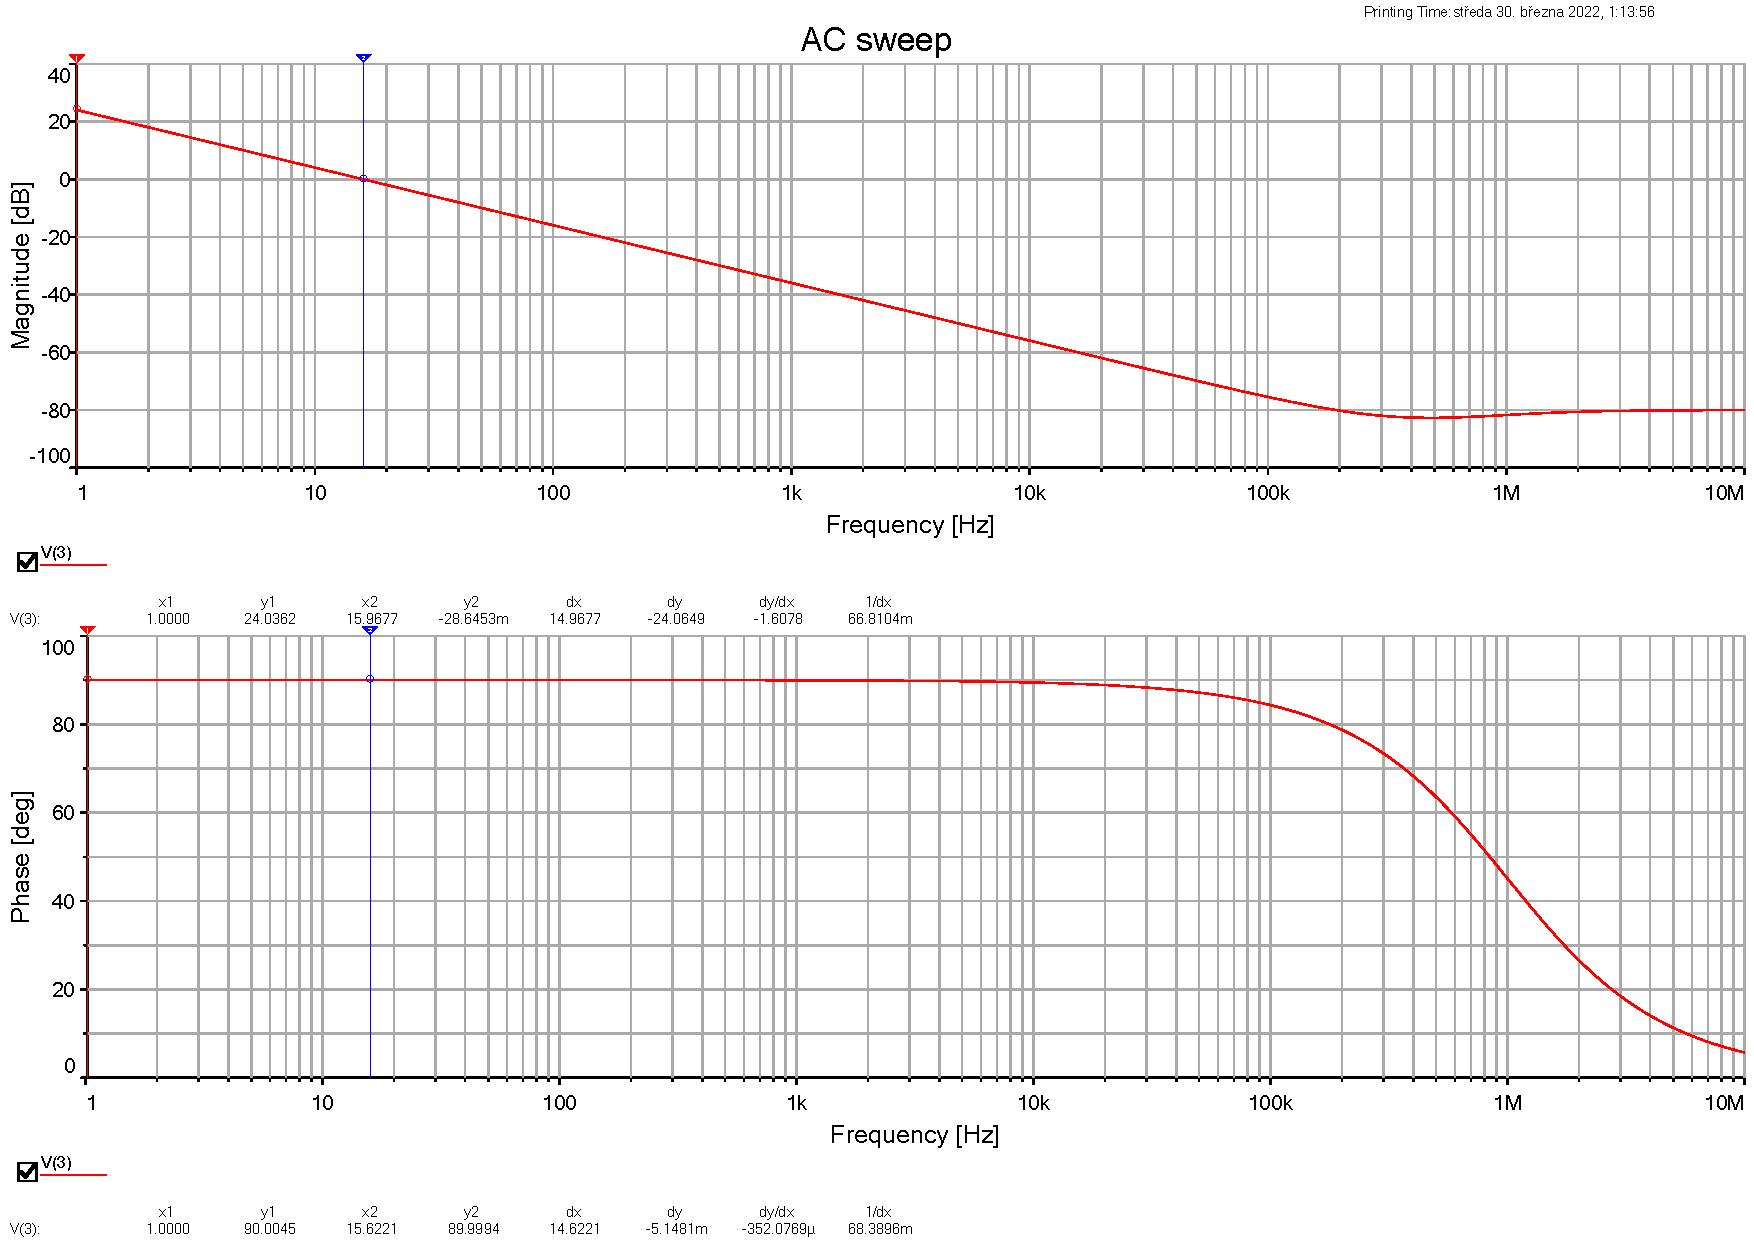
\includegraphics[width=0.92\linewidth]{bode_100.pdf}
    \caption{Frekvenční charakteristika pro $C_1 = 100 \si{\nano\farad}$}
    \label{fig:bode_100}
\end{figure}

\newpage
\section{Odezva na skok}

\begin{figure}[h!]
    \centering
    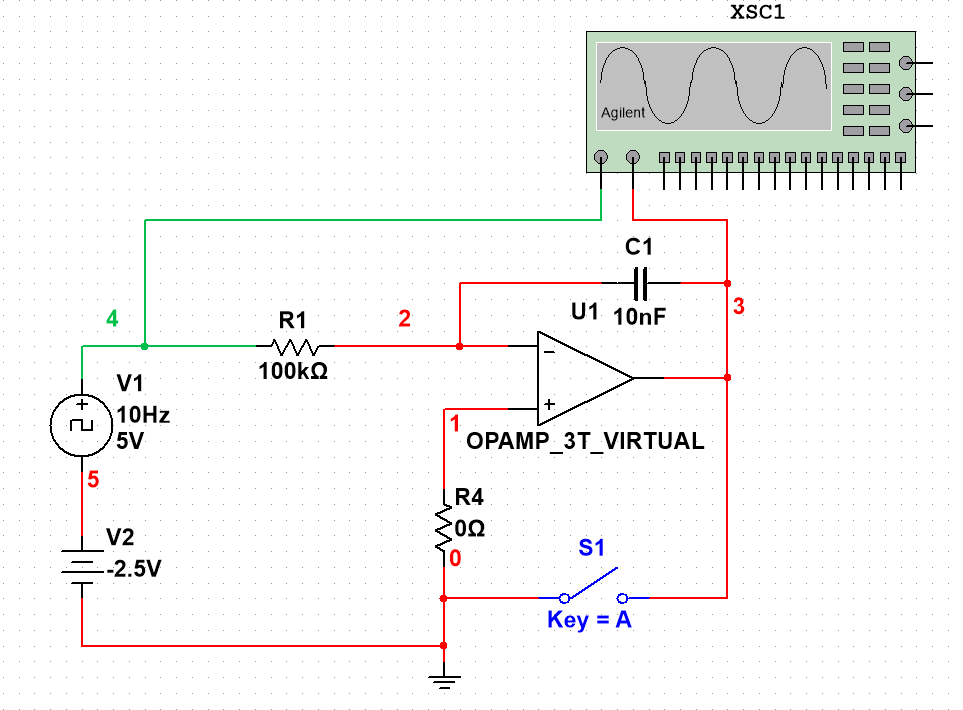
\includegraphics[width=0.7\linewidth]{odezva_na_skok_schema.png}
    \caption{Zapojení pro sledování odezvy na skok}
    \label{fig:skok_schema}
\end{figure}

S pomocí generátoru obdélníkového signálu a osciloskopu zapojeného dle schématu \ref{fig:skok_schema}
byly zachyceny časové průběhy vykreslené na obrázku \ref{fig:skok} pro $C_1 = 10 \si{\nano\farad}$.
Integrátor integruje po částech konstantní vstupní signál, výstupní napětí jsou tedy lineárně klesající či rostoucí funkce.
Ani při přibližování průběhů se nepodařilo pozorovat prudké skoky na začátku odezvy vlivem dopředného přenosu.
Spínač S1 je přidán pro umožnění občasného vynulování naintegrováného zbytkového napětí operačního zesilovače.

\begin{figure}[h!]
    \centering
    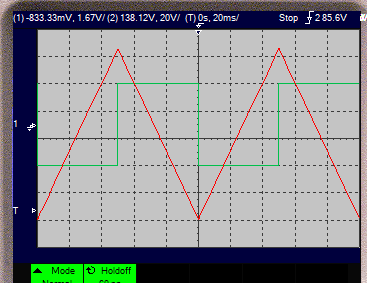
\includegraphics[width=0.6\textwidth]{odezva_na_skok.png}
    \caption{Odezva integračního zesilovače na skoky vstupu}
    \label{fig:skok}
\end{figure}

\newpage

\section{Lineární funkce na vstupu}

Integrálem lineární funkce je funkce kvadratická.
Na vstup intgerátoru s $C_1 = 10 \si{\nano\farad}$ byl připojen trojúhelníkový průběh napětí s velikostí $1 \si{\volt}_{\text{pk-pk}}$ se střídou 50 \% a periodou 1 s.
 Na výstupu byl pozorván signál složený po částech z parabol, jenž je na obrázku \ref{fig:kvadraticka}.

\begin{figure}[h!]
    \centering
    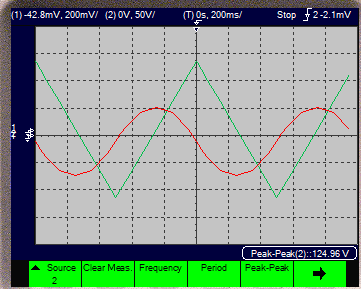
\includegraphics[width=0.6\textwidth]{kvadraticka.png}
    \caption{Integrál lineární funkce na vstupu integračního zesilovače}
    \label{fig:kvadraticka}
\end{figure}

Očekávanou velikost špička-špička signálu na výstupu lze vypočíst pomocí určitého integrálu vstupního signálu:
\begin{equation}
    U_{2_\text{pk-pk}} = \frac{1}{100 \si{\kilo\ohm} \cdot 10 \si{\nano\farad}} \int_0^{500 \si{\milli\second}} u_1(t) \text{d}t
    = 1000 \cdot 2 \cdot \int_0^{250 \si{\milli\second}} 2t \text{d}t = 2000 (250 \si{\milli\second})^2 = 125 V,
\end{equation}
což perfektně odpovídá skutečné hodnotě změřené osciloskopem na obrázku \ref{fig:kvadraticka}.

\end{document}

